%!TEX root = main.tex

\section{Introduction}


%A desirable video streaming protocol should maximize user-perceived video quality under dynamic network conditions.
%A key concern in video streaming is how to optimize video quality under fluctuating network bandwidth.
%On one hand, if the bandwidth is stable, one can maximize the quality (\eg high resolution, no rebuffering) by aggressively eliminating the pixel-level spatio-temporal redundancies.
%On the other hand, encoding the video too aggressively would make it hard to switch the quality level quickly enough to fully utilize the fluctuating bandwidth.
%A case-in-point of this tradeoff is DASH~\cite{??,??,??}, which recently took hold as the mainstream video protocol. 
%It balances the encoding efficiency and adaptation by splitting the video to fixed-length chunks (4-10 seconds) each encoded in discrete quality levels, allowing it to switch quality at chunk boundaries.

%The recent surge of \vr videos poses new challenges.
\vr videos are coming to age, with most major content providers roll out {\vr}video-based applications~\cite{??,??,??,??,??}.
At the same time, it has become clear that streaming \vr videos is much more challenging than streaming non-\vr videos.
To create an immersive experience, \vr videos must cover a larger area in high resolution than traditional videos without interruption~\cite{??}, which makes them much more bandwidth-intensive than traditional videos.
To put it into perspective, streaming a typical one-minute \vr video~\cite{give the url} as a regular video (\ie no head movement) takes only \fillme MB, whereas streaming it as a \vr video using state-of-the-art \vr streaming protocol takes \fillme MB, a \fillme$\times$ increase in bandwidth consumption.
%Although one can save bandwidth by streaming only the area facing the viewer, doing so would (1) require accurately tracking the viewpoint movements which itself is not trivial, and (2) force the encoder to use shorter video chunks (\eg one second) to keep up with the movements of the viewpoint, which significantly reduces the coding efficiency and thus increases the bandwidth consumption.

A key limiting factor in existing \vr video streaming solutions is that they have largely relied on the same QoE (quality of experience) model from non-\vr videos. 
They assume the impact of encoded quality of the video (\eg pixel-level distortion) on QoE is the same to traditional videos, which fundamentally limits the room for improvement of \vr videos.
%At a high level, the QoE model describes the correlation between how a video is presented to the viewer (\eg pixel-level differences to the original feed) and the user-perceived satisfaction, or QoE.
A notable exception is that the perceived QoE of a spatial area also depends on the region's distance to user's real-time viewpoint (\eg~\cite{??,??,??,??}), so one can save bandwidth by streaming only the area facing the viewer.
However, doing so would (1) require accurately tracking the viewpoint movements which itself is not trivial, and (2) force the encoder to use shorter video chunks (\eg one second) to keep up with the movements of the viewpoint, which significantly reduces the coding efficiency and thus increases the bandwidth consumption.
%But other than the above factor, the assumed QoE model remains largely the same, and this fundamentally limits the room for improvement of \vr videos.

In this paper, we argue that there are still many untapped opportunities to improve \vr video QoE with a {\em deeper understanding of how viewers perceive the \vr video quality}.
In addition to the conventional belief that \vr video QoE only depends on the encoded quality level and real-time viewpoint, 
%the 360\textdegree{} view depends only on its distance to the viewpoint and the encoded quality level, 
we found that the perceived quality of a \vr video is heavily influenced by several other factors unique to \vr videos---the {\em velocity} of the head movement, the {\em relative depth-of-field} of the viewpoint with respect to surrounding objects, and the {\em relative luminance} of the objects compared to those the user have just watched. 
%That is the viewport position and video quality, we found that a \vr video at least three reasons: the velocity of head movement, how the relative depth of the viewed objects, as well as the brightness of the objects compared to those the user have just watched. 
For instance, when shown the same video encoded at different quality levels, most viewers are very sensitive to even small quality distortion when the viewports are static, but the sensitivity drops sharply when they move the viewpoints (\eg shaking head or browsing the landscape). 
%Similarly, how sensitive the viewer is to a quality distortion depends greatly on how further/closer the object is or how much brighter/darker compared to objects that the viewer just saw.
Note that unlike in traditional videos, these factors are driven by ``user behaviors'' unique to \vr videos (see \S\ref{subsec:opportunities} for more discussions).


These findings
%that humans have only bounded sensitivity to quality degradation can 
have great implications for \vr video streaming. 
With a deeper understanding of how user perceive the video quality, the video streaming protocol can improve the perceived QoE by always raising the quality level by a perceivable amount, and save the bandwidth by always lowering the quality by an imperceivable amount. 
Based on an empirical study over \fillme \vr videos and \fillme actual viewers, we found that one can save \fillme\% bandwidth and \fillme\% less buffering ratio without any drop in perceived quality. (More discussions in \S\ref{subsec:potentials})


\begin{figure}
  \centering
  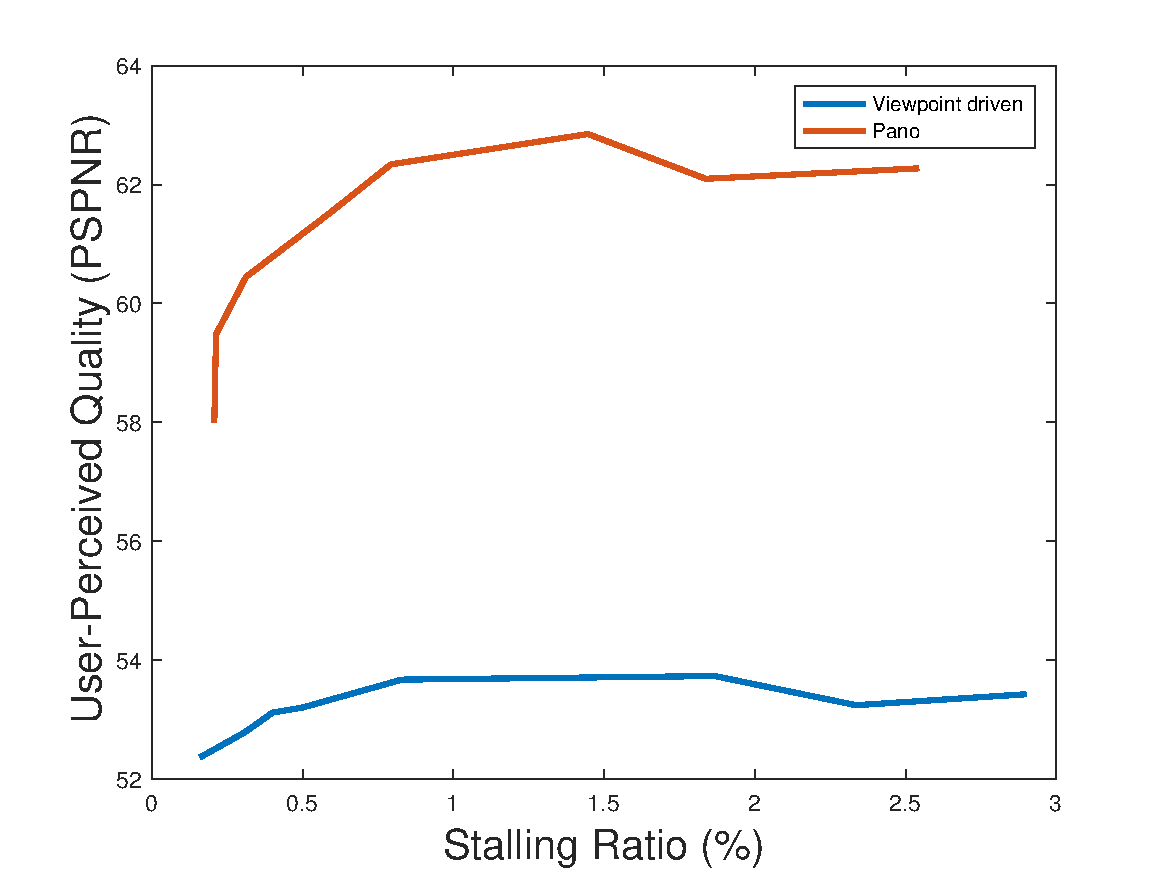
\includegraphics[width=3in]{images/intro-result.pdf}
  \caption{Performance of \name and the popular viewpoint-driven approach on \fillme \vrvideos and \fillme real-user viewpoint traces over an emulated link of \fillme($\pm$\fillme) Mbps.
  Full results are in \S\ref{sec:eval}.}
  \label{first_image}
\end{figure}

%\begin{figure}[t!]
%  \centering
%  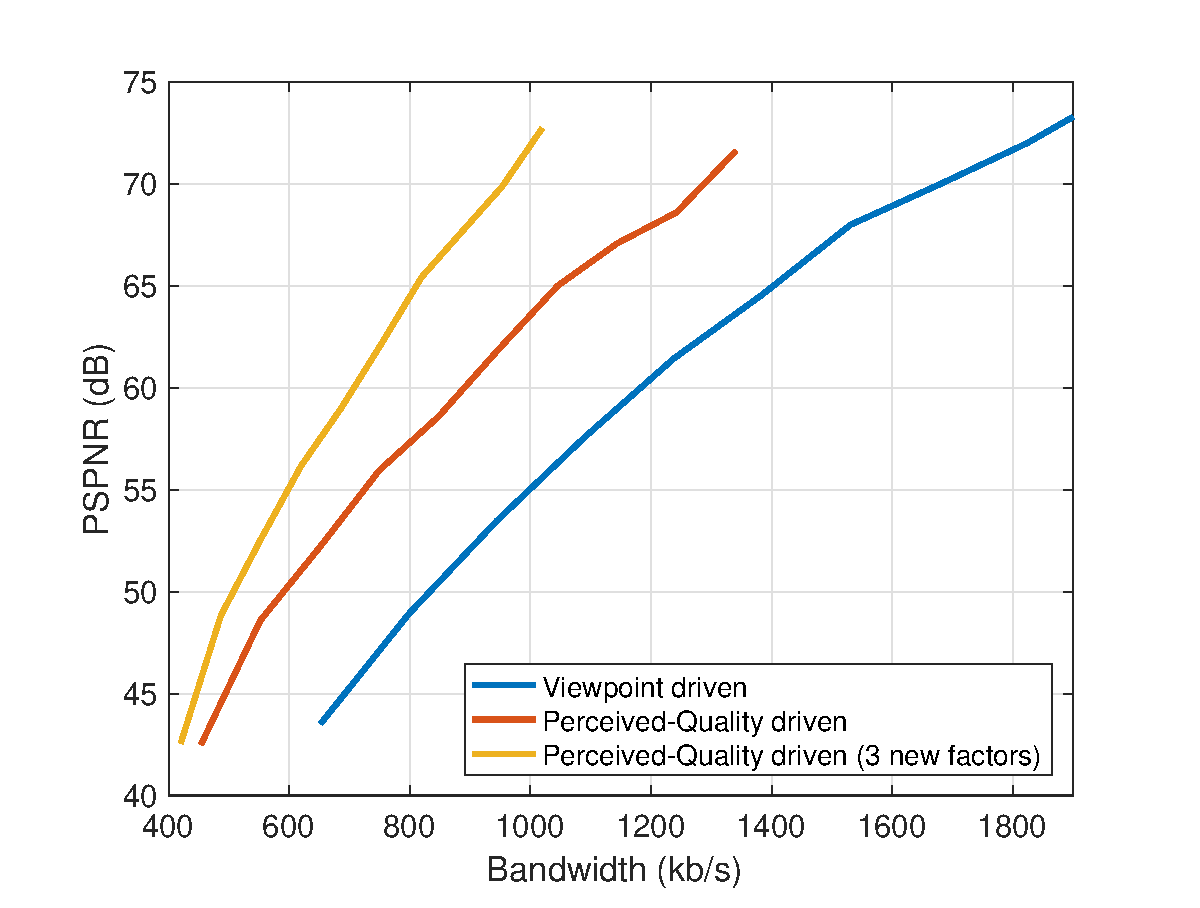
\includegraphics[width=2.5in]{images/improvement.eps}
%  \caption{Effectiveness of \name at reducing the bandwidth consumption and improving QoE. \jc{TODO. an example graph with two curves comparing \name and a canonical \vr video streaming protocol. }}
%  \label{fig:intro-improvement}
%  \end{figure}

The rationale behinds these opportunities is the fact that people have a limited span of attention.
For instance, as a viewer moves the viewpoint, it does increase the area that has to be streamed, but the viewer's ``per-pixel'' attention  (\ie sensitivity to quality distortion) drops as a result of having to spread the limited span of attention across a wider region.
We notice that similar ideas were explored in the context of video encoding with the concept of ``Just Noticeable Difference'' (JND)~\cite{??,??,??}---the minimal visual difference perceivable by humans, \eg viewers generally have larger JND when watching a more complex scene. 
However, conventional JND only models the content-level factors (it deals with static viewpoint), as opposed to the factors specific to the behaviors of \vr video viewers. 

This paper presents {\em \name}, an encoding and streaming system that optimizes the user-perceived QoE of \vr videos.
\name makes three contributions.

\vspace{0.1cm}
{\em First, \name presents a new QoE model that builds on the concept of JND to incorporate the new \vr video-specific factors (\S\ref{sec:jnd}).}
We ran an IRB-approved user study to quantify the impact of three factors---viewpoint velocity, relative depth-of-field, relative luminance---on viewer's sensitivity to quality degradation. 
In addition, we also take distance-to-viewpoint (commonly used in prior work) as a factor that affect the QoE.
We call the resulting JND model as {\em \vrjnd}. 
It can predict, for any given video and viewport trajectory, the minimal quality degradation likely be perceivable by the viewer.
An interesting empirical finding is that the new viewer-driven factors are largely independent to each other, which vastly simplifies the modeling of impact of multiple factors on JND, which would otherwise have to explore the space of an exponential number of combinations of multiple factors.
%Their likely independence might explained by \jc{what's the intuition here?}


\vspace{0.1cm}
{\em Second, \name proposes a novel spatial tiling mechanism to fully utilize the new JND model (\S\ref{sec:tiling}).}
To best utilize the proposed \vrjnd framework, the video encoding should allow different quality levels be applied to different regions in cognizant to the spatial distribution of \vrjnd values.
Unfortunately, we found the existing equal-sized square tiling (\eg 12$\times$6) often is far from ideal---a tile can be too coarse-grained (\ie unable to adapt the quality level according to \vrjnd) or too fine-grained (\ie low encoding efficiency).
%In fairness, the square tiling is designed to serve only one purpose of differentiating regions closer to the viewport center from the rest.

In contrast, \name splits the \vr video into square tiles of different sizes in order to roughly match the spatial boundaries of \vrjnd. 
Each tile is then encoded in multiple levels of quantization parameter, or QP, (like in prior work).
In some sense, this is a compromise between the more radical region-of-interest encoding (in which each object can be encoded differently) and the square tiling which simplifies the rendering of multiple tiles each with different QP levels.



\vspace{0.1cm}
{\em Finally, \name proposes an adaptive streaming protocol that is (a) robust to randomness of viewpoint movements, and (b) compatible with existing DASH protocols (\S\ref{sec:control}).}
At the first glance, allocating quality level based on user actions seems susceptible to randomness (\ie prediction errors) of the head movement. 
On the contrary, we show that it is possible to allocate quality level per tile in a way that tolerate substantial errors of viewpoint prediction. 
The reason stems from the fact that \vrjnd value of a region remains almost same for a range of actions (\eg \vrjnd remains the same as long as the viewpoint velocity is over a threshold), so what we need is to not to accurately predict the exact trajectory of the viewpoint, but rather the {\em range} of user actions.

Another practical challenge facing \name is that unlike traditional adaptive streaming, calculating \vrjnd requires real-time input from both the client (the real-time user trajectory) and the server (the pixel-level video content), making it incompatible to the mainstream DASH protocol which stream videos from stateless HTTP web servers. 
%on the server (\ie cannot be done by the client itself), so it is incompatible with the mainstream DASH protocols which stream videos from stateless HTTP web servers. 
%to determine the perceived quality of a chunk require some computation based on the video data on the server side, so in theory, it is incompatible with the mainstream DASH protocols which stream videos from stateless HTTP web servers.
%This is not a problem in non-\vr videos or existing \vr video protocols, because calculating the perceived quality of a chunk only depends on the available bandwidth and user viewport, both are locally accessible on the client side.
%However, the perceived quality in \vrjnd depends on the video content and user actions (\ie viewport trajectory and its projection), so the client cannot estimate the user-perceived quality without having the video content in the first place. 
%One approach to this conundrum is to let the video client upload the user action information to the server which then makes adaptation decisions, but this goes against DASH's HTTP-based architecture.
%Instead, in this work, we have taken a pragmatic stance to work within the constraints that have spurred the growth of video traffic---streaming videos from web servers over HTTP, like in DASH.
To run \name over the DASH protocol, we {\em decouple} the bitrate adaptation into an offline phase and an online phase.
In the offline phase, we pre-compute the best quality levels for only a few carefully picked possible values of the user action information (viewport trajectory and its projection), and send these estimates as part of the DASH metafile to the client at the beginning of a video session. 
%The basic idea is that it is possible to pre-compute the best quality levels for only a few carefully picked possible values of the user action information (viewport trajectory and its projection), and send these estimates as part of the DASH metafile to the client at the beginning of a video session. 
In the online phase, the client estimates the user action (as described above) and pick the quality level by the ``nearest neighbor'' among the user inputs that have been pre-computed. 
%The intuition behind pre-computing only a few user-action inputs is an empirical observation that in \vrjnd the impact of the user-action input is non-linear; \eg when the viewport movement speed is over some threshold, its impact on \vrjnd and the QP adaptation changes only marginally (probably because the viewer will be very insensitive).


\vspace{0.2cm}
We implemented a prototype of \name.
\jc{on what platform}
We ran a pilot study on one content provider with \fillme sessions. \jc{how many viewers? what types of videos?}

Our experiments show that \name can save 45\% bandwidth compared with state-of-art 360-video streaming solutions, without decrease of perceived quality.
\jc{add a line to describe the final user-rating based end-to-end experiments}

